\chapter{SpyREST: Automated RESTful API Documentation using an HTTP Proxy Server}


%\author{\IEEEauthorblockN{S M Sohan, Craig Anslow, and Frank Maurer}
%\IEEEauthorblockA{Department of Computer Science\\
%University of Calgary\\
%Calgary, Alberta T2N 1N4\\
%Email: \{smsohan, craig.anslow, frank.maurer\}@ucalgary.ca  }
%}
%\maketitle


\section{Abstract}
RESTful API documentation is expensive to produce and maintain due to the lack of reusable tools and automated solutions. Most RESTful APIs are documented manually and the API developers are responsible for keeping the documentation up to date as the API evolves making the process both costly and error-prone. In this paper we introduce a novel technique using an HTTP proxy server that can be used to automatically generate RESTful API documentation and demonstrate SpyREST, an example implementation of the proposed technique. SpyREST uses a proxy to intercept example API calls and intelligently produces API documentation for RESTful Web APIs by processing the request and response data. Using the proposed HTTP proxy server based technique, RESTful API developers can significantly reduce the cost of producing and maintaining API documentation by replacing a large manual process with an automated process.

%\IEEEpeerreviewmaketitle

%\begin{IEEEkeywords}
%RESTful API, Web API, Documentation, Automation, Example based documentation
%\end{IEEEkeywords}


\section{Introduction}
RESTful APIs, introduced by Fielding, are used as a primary interconnection mechanism among modern day web based systems \cite{Fielding_rest}. For example, the website of a restaurant can use the RESTful API from Twitter to show the latest tweets mentioning the restaurant so that prospective customers can read the experience shared by others. To allow others to use their APIs, Twitter and other RESTful API developers publish documentation describing different features of their RESTful API. The documentation of such RESTful APIs are often produced and maintained using a manual process that is expensive and error-prone.

API documentation for library APIs, such as Java Standard Edition, commonly leverage reusable tools such as JavaDoc. The documentation produced by such tools include description of objects and methods, with custom texts primarily sourced via comments in the source code. On the other hand, RESTful API documentation includes additional information such as HTTP headers, request parameters, request and response data in serialized formats (e.g. JSON, XML). Using comments for these additional information requires significant manual effort. There is a lack of reusable tools to automate the documentation process. This makes the task of producing RESTful API documentation a costly and error-prone one. API developers also need to publish and often maintain the documentation for multiple versions as the RESTful API evolves. This requires further manual effort.

To produce RESTful API documentation, the manual process used can be described as a six-step process as follows: 1) craft an example call to an API endpoint with required headers, URL parameters and request body, 2) make the call, 3) capture the response headers and data, 4) strip any confidential data from the captured information, 5) add custom descriptions to the captured data and 6) publish the API documentation. This six-step process is essentially repeated for all API endpoints that are documented. With \emph{SpyREST}, we have implemented an innovative solution to largely automate the aforementioned manual process of RESTful API documentation so that all but steps 1 and 5 are automated. Steps 1 and 5 are left to a manual process to allow for a pragmatic solution. Our solution relies on an HTTP proxy server to intercept example API calls to automatically capture all HTTP traffic. The collected data is then synthesized to present the documentation for RESTful APIs. SpyREST can generate documentation for all RESTful APIs irrespective of the technology used to implement the API since it leverages an HTTP proxy server.

The key contributions of our research are as follows: we discuss a list of requirements for tool development by analyzing related work to automate the RESTful API documentation process and present a new technique based on an HTTP proxy server to meet the requirements. We demonstrate an example implementation of the proposed technique that generates automated yet customizable, version-aware, collaboration enabled and reusable API documentation software as a service platform that can be used to generate and maintain documentation for any RESTful API. We present a case study of using SpyREST to compare the advantages of our proposed technique over existing solutions for RESTful API documentation.

The remainder of this paper is organized as follows: in the next section we discuss related work on API documentation. The requirements and implementation details of SpyREST is provided next. Then, we present a case study to demonstrate SpyREST in action. Finally, we discuss the implications and limitations of our work in the discussion section.


\section{Related Work} % (fold)
\label{sec:related_work}
\subsection{General API Documentation} % (fold)
\label{ssub:api_learnability}
Several papers have studied the documentation of APIs to recommend best practices that are also applicable to RESTful API documentation. Robillard et al. found that  developers faced severe obstacles learning new APIs due to inappropriate documentation and other learning resources \cite{Robillard_what_makes, Robillard_a_field_study}. Robillard recommended the following for API documentation: include good examples, be complete, support many complex usage scenarios, be conveniently organized, and include relevant design elements. Kuhn et al. discussed the importance of examples in API documentation \cite{Kuhn_on_designing}. Hoffman et al. recommended making the API example scenarios to be executable test cases so that a user can execute an API \cite{Hoffman_api_documentation}.

Nasehi et al. performed a case study based on StackOverflow discussions to find out what makes good code examples \cite{Nasehi_what_makes}. They recommended API developers to include examples in the API documentation and the use of wiki-like collaborative tools with online API documentation. Parnin et al. found that using social media gives API documentation readers a chance to engage with authors of the APIs \cite{Parnin_measuring}. Chen et al. recommended integrating crowdsourced frequently asked questions into API documents so that users can easily find relevant discussions when questions arise \cite{Chen_who_asked}. Subramanian et al. presented an automated approach to link API documentation of different Java and JavaScript libraries with code examples that are shared on StackOverflow \cite{Subramanian_live}.

Stepalina identified several advantages of software as a service (SaaS) based solutions for API documentation systems such as, cost effective yet powerful, platform agnostic and high accessibility, improved document quality, content re-use, automated tools, and organization of robust and scalable documentation process \cite{Stepalina_saas}. Several tools exist that help automatic generation of API documentation for local APIs such as JavaDoc\footnote{http://www.oracle.com/technetwork/java/javase/documentation/index-jsp-135444.html}, RDoc\footnote{http://rdoc.sourceforge.net/}, Jadeite \cite{Jadeite}. While these tools have been proven to work for local library APIs, they have limited applicability for documenting RESTful APIs because HTTP specific information are not natively supported by these tools.

\subsection{RESTful API Documentation} % (fold)
\label{sub:restful_api_documentation}

Several related work proposed specifications for RESTful APIs. Maleshkova et al. found that a lack of a standard format to document Web APIs and manual documentation causes confusions about how to use the APIs for different use cases \cite{Maleshkova_investigating}. Espinha et al. observed that most RESTful APIs are documented manually by API developers making the documentation a less reliable one \cite{Espinha_web}. Danielsen et al. presented a vocabulary for documenting RESTful Web APIs called Web Interface Language (WIfL) \cite{Danielsen_validation}. Verborgh et at. presented RESTdesc, a Resource oriented and Hyper-link based specification for describing RESTful APIs \cite{Verborgh_functional}. Mangler et al. presented RDDL, an XML based specification for describing RESTful APIs \cite{Mangler_rddl}. Kopecky´ et al. presented hRESTS, a machine readable micro-format to describe RESTful APIs that use an alternate representation compared to WIfL \cite{Kopecky_hrests}. Ning et al. presented OmniVoke, a RESTful API based invocation engine that provides an abstraction layer for RESTful API calls to multiple APIs that follow different conventions \cite{Ning_omnivoke}. Manual configuration is required to generate these aforementioned specifications for RESTful APIs. Myers et al. recommended providing a consistent look-and-feel with explanation for the starting points and an overall map comprising of both text and diagrams, providing a browsing experience with breadcrumb trail following a hierarchy, an effective search interface, providing example code and a way to exercise the examples online without writing code \cite{Myers_study}.

In addition to the research community, there are several custom RESTful API specification formats that are observed in the industry such as, Swagger\footnote{https://github.com/swagger-api/swagger-spec/blob/master/versions/2.0.md}, RAML\footnote{http://raml.org/spec.html}, and Blueprint\footnote{https://github.com/apiaryio/api-blueprint}. In addition to producing RESTful API documentation, there are SaaS based tools providers that can be used to publish the documentation and auto generate API client code for RESTful APIs that are described using one of these formats. To use these tools to generate HTML based RESTful API documentation, API developers need to manually construct the intermediate documentation format such as Swagger, Blueprint, RAML, etc. since there is no automated tool to produce this.
% subsubsection restful_api_specification (end)


\section{SpyREST} % (fold)
\label{sec:spyrest}

\subsection{Requirements} % (fold)
\label{sub:spyrest_requirements}

The following list of requirements for SpyREST, R1-7, in priority order, is derived from analyzing the aforementioned related work and current API documentation practices as observed in the industry:

  \textbf{R1 - Automated RESTful API documentation}: RESTful APIs are either documented manually or using custom tools to partially automate the process. The primary requirement for SpyREST is to find a cost-effective approach to automate RESTful API documentation.

  \textbf{R2 - Example based}: As discussed in the related work section, several authors have emphasized including example scenarios with API documentation can help users understand how to use an API \cite{Robillard_what_makes, Kuhn_on_designing, Hoffman_api_documentation,Nasehi_what_makes}. SpyREST generated API documentation needs to include example scenarios.

  \textbf{R3 - Executable documentation}: In addition to including examples, SpyREST also needs to allow users to execute the example scenarios so that they can try the API features without having to write code \cite{Hoffman_api_documentation, Myers_study}.

  \textbf{R4 - Version awareness}: SpyREST needs to allow API developers to publish documentation for multiple versions of a Web API as it evolves. The following comment from an API client developer of Stripe, an online payment processing company, shows the importance of a version-aware documentation tool\footnote{\url{https://groups.google.com/a/lists.stripe.com/forum/\#!searchin/api-discuss/version/api-discuss/li4PyVcweiw/NT9SFTtF-vQJ}}
:
  \small
  \begin{quotation}
   ``Does the full API documentation only reflect the current version of the
    API?  Is there a way to access the API docs for outdated versions? ...That would be very helpful. When you are trying to upgrade from one version to another it's impossible to know the implementation differences...''
  \end{quotation}
  \normalsize

  \textbf{R5 - Customizable}: It is important to customize the overview information about how to use an API to reduce API learning obstacles and describe complicated business rules\cite{Robillard_what_makes}. SpyREST needs to allow API developers to add customized content to auto generated RESTful API documentation.

  \textbf{R6 - Reusable}: SpyREST needs to work as a reusable platform so that multiple REST API documentations can be generated and published on a single platform to get the advantages of a SaaS platform \cite{Stepalina_saas}.

  \textbf{R7 - Collaborative}: SpyREST needs to allow people to collaborate on the API documentation so that questions and answers about APIs can coexist with the API documentation to to overcome the knowledge fragmentation \cite{Chen_who_asked}.


\subsection{Design} % (fold)
From our research, we identified an HTTP proxy server based solution as a novel approach for generating RESTful API documentation meeting requirements R1-7. Our approach works as follows: API developers make example API calls using a proxy $\longrightarrow$ the proxy records and processes HTTP traffic $\longrightarrow$ a Web App generates RESTful API documentation. SpyREST, an example implementation of this approach\footnote{\url{https://github.com/smsohan/demo_paper/raw/master/SpyREST_tool_demo.pdf}}, is composed of three main components as follows:

\textbf{The Spy:} The Spy component in SpyREST is an HTTP proxy server. The Spy is named so because it records the HTTP traffic for example API calls that are made using it as a proxy server. For example, when using Spy as an HTTP proxy to make the following HTTP request:

\footnotesize
\begin{description}
  \item[Method] GET
  \item[URL] https://api.github.com/repositories?since=100
  \item[Headers] accept: application/vnd.github.v3+json
\end{description}
\normalsize
that produces the following response:
\footnotesize
\begin{description}
  \item[Headers] status: 200 OK \\
content-type: application/json; charset=utf-8 \\
...
  \item[Body]
\begin{lstlisting}
[
  {
    "id": 1,
    "name": "grit",
    "full_name": "mojombo/grit",
    ...
  }
]\end{lstlisting}
\end{description}
\normalsize
Spy automatically saves the raw request and response data with HTTP headers. Additionally, the Spy synthesizes the data and saves the following meta data about this example API call:

\footnotesize
\begin{tabular}{r p{0.55\linewidth}}
  version & v3 \\
  resource & repositories \\
  action & GET /repositories \\
  query & since: 100 \\
  strippedResponseBody & a subset of the response body \\
  description & blank \\
  digest & base64 hash value of the version, resource, url and description \\
  requiresAuth & false \\
  apiToken & blank, used when a SpyREST API token is provided \\
  userId & blank, used when a user is found for given apiToken \\
\end{tabular}
\normalsize

As shown in this example, the version ``v3'' is automatically detected by parsing the accept request header. Next, the resource field is also auto detected as ``repositories'' by parsing the request URL. The action ``GET /repositories'' is automatically detected by combining the request HTTP method with request path. The strippedResponseBody field automatically saves a shorter version of the actual response where large response body is truncated to a smaller one to reduce noise from the generated documentation. These meta fields allow SpyREST to structure the example API calls for a given API host in a hierarchical model as follows: an APIHost (e.g. GitHub.com) has many APIVersions (e.g. v3), each APIVersion has many APIResources (e.g. repositories), each APIResource has many APIActions (e.g. GET /repositories), and each APIAction has many APIExamples.

\begin{figure*}[!tbh]
  \centering
  \begin{subfigure}[t]{0.4\textwidth}
    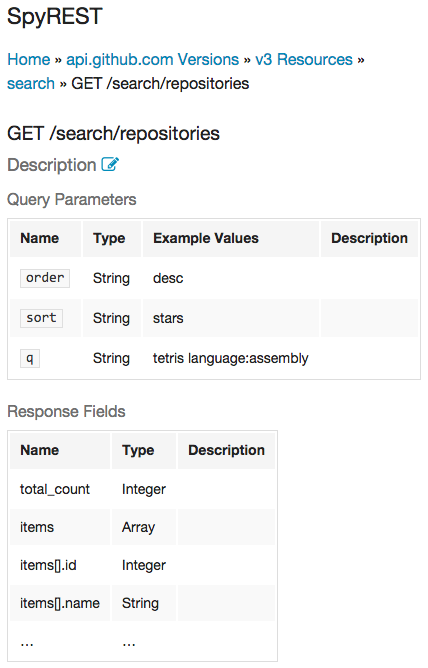
\includegraphics[width=\linewidth]{spyrest_header.png}
    \caption{API documentation summary section}
    \label{fig:summary}
  \end{subfigure}
  \begin{subfigure}[t]{0.5\textwidth}
    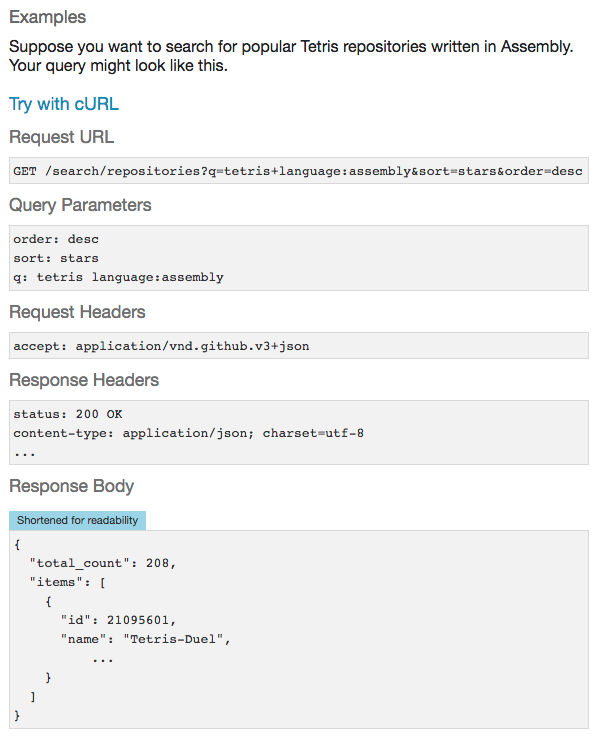
\includegraphics[width=\linewidth]{spyrest_examples.png}
    \caption{API documentation examples section}
    \label{fig:examples}
  \end{subfigure}
  \caption{SpyREST Screen shots showing auto generated API documentation}
  \label{fig:spyrest_screenshots}
\end{figure*}

\textbf{The Database:} The database component saves the data that is captured by the Spy and the Web App. The Spy saves the recorded data about the API examples and the auto-computed meta data in the database. The Web App saves data about SpyREST users and custom modifications on auto-generated API documentation on the same database.

\textbf{The Web App:} The Web App component further processes and presents auto generated documentation that is captured by Spy in the database. The Web App also allows the API developers to edit or add custom content to the auto generated documentation. The source code for both the Spy and Web App components are released as open source projects.

\subsection{Features} % (fold)

Now that we have explained the design and implementation of SpyREST, we discuss how SpyREST meets the aforementioned requirements R1-7.

\textbf{R1 - Automated RESTful API documentation:} The work flow for automated RESTful API documentation can be explained by the following steps: 1) API developer uses the Spy HTTP proxy to run example API calls, 2) The Spy records example API calls, 3) The Spy extracts meta information about the API call, 4) The Web App displays the auto generated documentation, 5) API developers can optionally customize the auto generated documentation.

Fig \ref{fig:spyrest_screenshots} shows screen shots (shortened) from SpyREST auto generated documentation that is solely based on an example API call to URL \url{https://api.github.com/search/repositories?q=tetris+language:assembly&sort=stars&order=desc} with a custom header ``x-spy-rest-description'' to provide the short description for the example.

The auto generated API documentation features two sections, a summary section as shown in Fig. \ref{fig:summary} and an examples section as shown in Fig. \ref{fig:examples}. The summary section includes breadcrumbs to show hierarchy of the API objects related to each API action to help API client developers easily navigate the API documentation. This section also includes three tables that display the structure of query parameters, and request and response payloads. In addition to the structure, automated type detection is used to show the data type and example values for each field in these tables. The examples section on the API documentation shows all the recorded API examples for a given API action. For each example, it shows a description, the request URL, query parameters, and request and response headers and bodies. Spy filters out the ``authorization'' request header before saving the examples in the database and the documentation rendered by the Web App displays this header with a placeholder text as ``FILTERED''.

\textbf{R2 - Example based:} SpyREST generated RESTful API documentation includes both the structure of the API objects and concrete examples for different use cases. The API examples are annotated with user provided descriptions through a custom HTTP request header ``x-spy-rest-description'' that is otherwise hard to automatically infer. To record the examples in SpyREST, any REST API client can be used as long as it supports an HTTP proxy to call the API.

\textbf{R3 -  Executable documentation:} SpyREST keeps a copy of the API request information including URL, headers and request body. As a result, SpyREST can also recreate the example API calls that can be executed by users of the generated API documentation. SpyREST automatically generates executable test cases that can be run using cURL\footnote{http://curl.haxx.se/}.

\textbf{R4 - Version awareness:} SpyREST allows API developers to publish the documentation for multiple versions of their RESTful APIs. To organize API documentation and examples under multiple versions, SpyREST has an automatic version detection algorithm that parses the ``accept'' request header or the URL. The auto version detection algorithm can be suppressed by specifying the version in the custom ``x-spy-rest-version'' header when running example API calls through the Spy.

\textbf{R5 - Customizable:} SpyREST allows API developers to modify and add custom free-form contents to the auto generated summary section of the documentation using Markdown\footnote{\url{http://en.wikipedia.org/wiki/Markdown}} syntax. Custom content can be used to provide overview information and explain complicated business rules about the APIs that are not derivable from simply synthesizing the examples. We consider this as a pragmatic solution to augment manual effort with the largely automated solution to the RESTful API documentation effort. The custom edits are persisted in the database and are not overridden when the API examples are replayed unless the user decides to revert back to automated summaries.

\textbf{R6 - Reusable:} SpyREST relies on an HTTP proxy to auto generate RESTful API documentation. To feed SpyREST with data, any REST API client can be used as long as it supports using a proxy server. This technology agnostic feature allows SpyREST to be a reusable RESTful API documentation tool. SpyREST is offered as a SaaS tool at \url{http://spyrest.com} that can be used to auto-generate and publish documentation of multiple RESTful APIs. For APIs where a SaaS solution is not acceptable, SpyREST can also be installed and used as a self-hosted solution. Because SpyREST is an open-source application, users can modify the source to support any unique requirements that are not supported by SpyREST.

\textbf{R7 - Collaborative:} SpyREST allows the API developers to comment and discuss API related questions with API client developers right next to the documentation so that crowdsourced documentations can coexist with the officially published API documentation. Each API documentation page on SpyREST features its own discussion thread to help users easily locate relevant information.

\section{SpyREST Case Study}
\label{sec:case_study}
In this section we discuss a case study of using SpyREST to auto generate documentation for 25 API actions randomly sampled from three RESTful API providers. These 25 API APIs are documented using 272 lines of code\footnote{\url{https://github.com/smsohan/spyrest_examples}}. These three API providers are: GitHub.com, KISSMetrics.com (Online analytics tool), and LiquidPlanner.com (Online project management tool).

\subsection{SpyREST Documentation vs. Official Documentation} % (fold)
\label{sub:spyrest_vs_official_documentation}

We found SpyREST generated documentation for 5 of the 25 API actions from the case study included fields that are found from actual API responses but not included in their official documentation. For example, the SpyREST generated documentation for Github \texttt{GET /notifications} API action included 34 additional fields, such as: \texttt{forks\_url, keys\_url, collaborators\_url}, and 29 more that were not mentioned in the official API documentation even though actually returned as API response. Similarly, the official documentation for GitHub.com \texttt{GET /search/code} API action did not include the \texttt{releases\_url} API response field. Official documentation of KISSMetrics.com \texttt{GET core/accounts} and \texttt{GET core/accounts/:account\_id} API actions did not mention the \texttt{data} field that is found in the actual response as documented by SpyREST. The official documentation for \texttt{GET /api/account} action on LiquidPlanner.com did not mention the fields \texttt{workspaces, last\_workspace\_id, and disabled\_workspaces\_count} that were included in the SpyREST documentation. These examples show the error-prone nature of a manual process that requires API developers to ensure the documentation is updated to reflect any change in the API. We consider the proxy based solution to solve this problem since the API documentation can be updated by replaying the example API calls.

The official documentation of these three API providers did not include integrated collaboration features. We found 172 unanswered questions out of 662 questions with the tag \texttt{github-api} on StackOverflow.com. We found 123 questions about LiquidPlanner API on their developer forum that are not linked to officially generated documentation published as a PDF file. On StackOverflow.com, we found 4 unanswered questions out of 9 questions on KISSMetrics API. SpyREST provides the collaboration features with auto generated API documentation so that API developers and users can discuss and locate related discussions when browsing RESTful API documentation on a single web interface. SpyREST includes executable API examples, support for multiple versions and presents the auto generated documentation for different RESTful APIs using a consistent look and feel that are not provided by these studied APIs.

\section{Discussion}
RESTful API documentation is expensive, error-prone, and often incomplete because of the manual effort involved in the process. Our core contribution is a novel approach where an HTTP proxy server is used to largely automate the process for RESTful API documentation. There is a lack of tool support for automatically generating documentation of RESTful APIs. We presented SpyREST as an example implementation of the HTTP proxy server based solution to fill this need. The requirements for SpyREST are derived from analyzing the existing literature and industry practices as well as our own professional experiences developing RESTful APIs and their documentation. In the literature, several papers provided lists of recommendations for API documentation based on studying the existing tools and techniques and feedback collected from API developers. We found a lack of available tool support to generate RESTful API documentation following those recommendations and designed SpyREST to provide a solution. As a result, SpyREST features automated documentation with executable examples, customizable contents, collaboration, version awareness and reusability to provide a ready to use tool support for RESTful API documentation following the recommendations.

The novel approach of using an HTTP proxy sever offers some unique benefits over existing tools from academia and industry. For example, tools that rely on user provided comments on source code and code inspection, such as JavaDoc, require the user to write formatted comments that are often applicable to a single programming language. The comments are not executable, and manual effort is required to ensure the comments and the API that it describes are kept in sync. SpyREST generated documentation can reflect the latest information since the documentation is generated after executing the example API calls. The verbose nature of RESTful API documentation makes it difficult to write and maintain the documentation as comments in source code. Using an HTTP proxy server, SpyREST offers a language agnostic solution so that RESTful APIs written in any programming language can be documented using a single tool.

Another key feature of SpyREST is the shared platform for publishing RESTful API documentation. A similar shared platform is provided by several other tools such as Swagger, Blueprint. We identify the key advantage of SpyREST over these tools to be the fact that SpyREST relies on example API calls instead of relying on a custom API specification that are required by these tools. The suggested API specifications can be used to define the structure of API objects but do not capture examples of API usage. The work flow for using these API specification formats can be described as follows: (1) execute example API calls $\longrightarrow$ (2) manually generate API specification $\longrightarrow$ (3) automatically generate API documentation. SpyREST does not rely on any custom API specification, so the associated manual effort can be largely avoided resulting in a smaller work flow as follows: (1) execute example API calls $\longrightarrow$ (2) automatically generate API documentation. We consider this process to be a cost effective approach for APIs with several endpoints or APIs that evolve. Unlike other available SaaS only solutions such as Swagger, and Blueprint, SpyREST can be used both as a SaaS and a self-hosted platform. The self-hosted mode can be used for documenting internal RESTful APIs that cannot be released on the internet or modifying the open-sourced code of SpyREST to fit unique API specific needs. We have demonstrated using SpyREST with automated test code. Using the test code helps automatically testing different use-case scenarios of the API actions in addition to generating the API documentation.

While SpyREST offers an automated solution for documenting RESTful APIs, API developers can customize the auto generated content. Several researchers have identified the need for rich content comprising of text and diagrams to explain complex business rules about APIs. To achieve this goal, we consider augmenting auto generated documentation with user contributed documentation, when necessary, to provide a pragmatic solution. To summarize, from our example implementation of SpyREST and the case-study, we have shown the advantages of the proposed HTTP proxy server based solution over the existing techniques for RESTful API documentation.

\subsection{Threats to Validity} % (fold)
\label{sub:threats_to_validity}

\textbf{Internal Threats.} Our proposed technique uses an HTTP proxy server that can only intercept and record the data when it is either in clear text or trusted to be decrypted by SpyREST. Because SpyREST can be used as a shared platform, any secrets used in the example API calls get decrypted in memory, even though not saved by SpyREST. To overcome these threat, we recommend API developers to use disposable secrets so that the secrets used to run an API call are valid for a single API call. For use cases where this is unacceptable, the self-hosted mode can be used as an alternative. SpyREST currently only supports JSON based APIs for their widespread use among popular RESTful APIs such as Twitter, Facebook, Google Maps.

\textbf{External Threats.} We used SpyREST to auto generate documentation for APIs randomly sampled from three RESTful API providers as a proof of concept and found the proxy server based solution met the requirements R1-7. Further evaluation is needed involving a larger set of RESTful APIs to evaluate the effectiveness of the proposed technique of using an HTTP proxy server for RESTful API documentation.

\section{Conclusion}
In this paper, we have presented a novel technique of using an HTTP proxy server to automate the RESTful API documentation process that otherwise requires a largely manual process. The proxy server based solution supports integrated features such as automated RESTful API documentation with executable example API calls, support for multiple versions, customization and collaboration that are offered both as a SaaS and self-hosted platforms. These features have been recommended by existing research on the documentation of APIs. Overall, we conclude that a proxy server based approach shows a pragmatic solution to the RESTful API documentation problem. In the future, we will perform a qualitative user study involving RESTful API developers to evaluate the effectiveness about the aforementioned HTTP proxy based RESTful API documentation approach.
\bibliographystyle{IEEEtran}
\bibliography{IEEEabrv,spy_rest/references}

